% !TEX TS-program = xelatex
% !TEX encoding = UTF-8 Unicode
% 
% © 2016 Moritz Brinkmann, CC-by-sa
% http://latexkurs.github.io

\documentclass[11pt,oneside,a4paper]{standalone}


\usepackage{mathtools}

\usepackage{tikz}
\usetikzlibrary{matrix}
\usetikzlibrary{arrows}



\DeclareMathOperator{\Coker}{Koker}
\DeclareMathOperator{\Ker}{Ker}


\begin{document}


  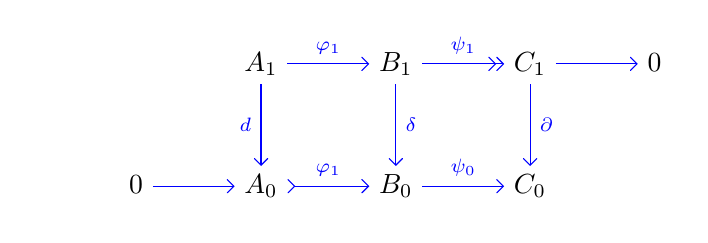
\begin{tikzpicture}[>=angle 90]
    \matrix[matrix of math nodes,
    row sep=3em, column sep=3em,,
    text height=1.5ex, text depth=0.25ex]
    {
      &&|[name=A1]| A_1 &|[name=B1]| B_1 &|[name=C1]| C_1 &|[name=01]| 0 \\
      &|[name=00]| 0 &|[name=A0]| A_0 &|[name=B0]| B_0 &|[name=C0]| C_0 \\ 
    };
    \draw[>->,font=\scriptsize,blue]
      (A0) edge node[auto] {$\varphi_1$} (B0);
    \draw[->>,font=\scriptsize,blue]
      (B1) edge node[auto] {$\psi_1$} (C1);
    \draw[->,font=\scriptsize,blue]
      (A1) edge node[auto] {$\varphi_1$} (B1)
      (B0) edge node[auto] {$\psi_0$} (C0)
      (A1) edge node[left] {$d$} (A0)
      (B1) edge node[auto] {$\delta$} (B0)
      (C1) edge node[auto] {$\partial$} (C0)
      (C1) edge (01)
      (00) edge (A0);
  \end{tikzpicture}




\end{document}
